% abtex2-modelo-artigo.tex, v-1.9.2 laurocesar
% Copyright 2012-2014 by abnTeX2 group at http://abntex2.googlecode.com/ 
%

% ------------------------------------------------------------------------
% ------------------------------------------------------------------------
% abnTeX2: Modelo de Artigo Acadêmico em conformidade com
% ABNT NBR 6022:2003: Informação e documentação - Artigo em publicação 
% periódica científica impressa - Apresentação
% ------------------------------------------------------------------------
% ------------------------------------------------------------------------

\documentclass[
	% -- opções da classe memoir --
	article,			% indica que é um artigo acadêmico
	11pt,				% tamanho da fonte
	oneside,			% para impressão apenas no verso. Oposto a twoside
	a4paper,			% tamanho do papel. 
	% -- opções da classe abntex2 --
	%chapter=TITLE,		% títulos de capítulos convertidos em letras maiúsculas
	%section=TITLE,		% títulos de seções convertidos em letras maiúsculas
	%subsection=TITLE,	% títulos de subseções convertidos em letras maiúsculas
	%subsubsection=TITLE % títulos de subsubseções convertidos em letras maiúsculas
	% -- opções do pacote babel --
	english,			% idioma adicional para hifenização
	brazil,				% o último idioma é o principal do documento
	sumario=tradicional
	]{abntex2}


% ---
% PACOTES
% ---

% ---
% Pacotes fundamentais 
% ---
\usepackage{lmodern}			% Usa a fonte Latin Modern
\usepackage[T1]{fontenc}		% Selecao de codigos de fonte.
\usepackage[utf8]{inputenc}		% Codificacao do documento (conversão automática dos acentos)
\usepackage{indentfirst}		% Indenta o primeiro parágrafo de cada seção.
\usepackage{nomencl} 			% Lista de simbolos
\usepackage{color}				% Controle das cores
\usepackage{graphicx}			% Inclusão de gráficos
\usepackage{microtype} 			% para melhorias de justificação
% ---
		
% ---
% Pacotes adicionais, usados apenas no âmbito do Modelo Canônico do abnteX2
% ---
\usepackage{lipsum}				% para geração de dummy text
% ---
		
% ---
% Pacotes de citações
% ---
\usepackage[brazilian,hyperpageref]{backref}	 % Paginas com as citações na bibl
\usepackage[alf]{abntex2cite}	% Citações padrão ABNT

\usepackage{listings}
\lstset{
  basicstyle=\small,
  columns=fullflexible,
  breaklines=true,
  postbreak=\raisebox{0ex}[0ex][0ex]{\color{red}$\hookrightarrow$\space}
  }


% ---

% ---
% Configurações do pacote backref
% Usado sem a opção hyperpageref de backref
\renewcommand{\backrefpagesname}{Citado na(s) página(s):~}
% Texto padrão antes do número das páginas
\renewcommand{\backref}{}
% Define os textos da citação
\renewcommand*{\backrefalt}[4]{
	\ifcase #1 %
		Nenhuma citação no texto.%
	\or
		Citado na página #2.%
	\else
		Citado #1 vezes nas páginas #2.%
	\fi}%
% ---

% ---
% Informações de dados para CAPA e FOLHA DE ROSTO
% ---
\titulo{Relatório do projeto de Computação Gráfica}
\autor{Antônio Adelino \and Armstrong Lohãns \and Carlos Antônio}
\local{Brasil}
\data{2019}
% ---

% ---
% Configurações de aparência do PDF final

% alterando o aspecto da cor azul
\definecolor{blue}{RGB}{41,5,195}

% informações do PDF
\makeatletter
\hypersetup{
     	%pagebackref=true,
		pdftitle={\@title}, 
		pdfauthor={\@author},
    	pdfsubject={Modelo de artigo científico com abnTeX2},
	    pdfcreator={LaTeX with abnTeX2},
		pdfkeywords={abnt}{latex}{abntex}{abntex2}{atigo científico}, 
		colorlinks=true,       		% false: boxed links; true: colored links
    	linkcolor=blue,          	% color of internal links
    	citecolor=blue,        		% color of links to bibliography
    	filecolor=magenta,      		% color of file links
		urlcolor=blue,
		bookmarksdepth=4
}
\makeatother
% --- 

% ---
% compila o indice
% ---
\makeindex
% ---

% ---
% Altera as margens padrões
% ---
\setlrmarginsandblock{3cm}{3cm}{*}
\setulmarginsandblock{3cm}{3cm}{*}
\checkandfixthelayout
% ---

% --- 
% Espaçamentos entre linhas e parágrafos 
% --- 

% O tamanho do parágrafo é dado por:
\setlength{\parindent}{1.3cm}

% Controle do espaçamento entre um parágrafo e outro:
\setlength{\parskip}{0.2cm}  % tente também \onelineskip

% Espaçamento simples
\SingleSpacing

% ----
% Início do documento
% ----
\begin{document}

% Retira espaço extra obsoleto entre as frases.
\frenchspacing 

% ----------------------------------------------------------
% ELEMENTOS PRÉ-TEXTUAIS
% ----------------------------------------------------------

%---
%
% Se desejar escrever o artigo em duas colunas, descomente a linha abaixo
% e a linha com o texto ``FIM DE ARTIGO EM DUAS COLUNAS''.
% \twocolumn[    		% INICIO DE ARTIGO EM DUAS COLUNAS
%
%---
% página de titulo
\maketitle


% ]  				% FIM DE ARTIGO EM DUAS COLUNAS
% ---

% ----------------------------------------------------------
% ELEMENTOS TEXTUAIS
% ----------------------------------------------------------
\textual

% ----------------------------------------------------------
% Introdução
% ----------------------------------------------------------
\section*{Introdução}
\addcontentsline{toc}{section}{Introdução}

Como projeto de disciplina da cadeira de Computação Gráfica do período de 2019.2 da Universidade 
Federal Rural de Pernambuco - Unidade Acadêmica de Garanhuns, ministrada pelo 
professor Doutor Ícaro Lins Leitão da Cunha, foi solicitado a nós alunos a implementação de um
projeto que envolvesse teorias expostas na disciplina, projeto o qual deveria ser codificado 
usando a biblioteca OpenGl na linguagem C ou Python.

Partindo dessas especificações iniciais codificamos a representação 3D de um boneco de neve, o qual
tem em sua implementação conceitos vistos em aula como a criação da estutura de armazenamento dos
elementos visuais, aplicação de luz e sombra, além de suportar também a interação com o usuário.

Com isso, o presente trabalho busca relatar e ilustrar o que foi implementado por nós, tendo
como principal finalidade descrever o processo de codificação e mostrar detalhadamente partes do código.

% ----------------------------------------------------------
% Seção de explicações
% ----------------------------------------------------------
\section{Código}

\subsection{Estrutura de armazenamento}

Dado que escolhemos modelar a imagem de um boneco de neve, escrevemos a estrutura
mostrada no Listing 1 para a criação da estrutura inicial de dados responsavel pela construção da 
estrutura do boneco de neve.  

\begin{lstlisting}[language=Python, caption=Estrutura de armazenamento]
   
   # Metodo para definir a estrutura do boneco
   def desenharBonceDeNeve():
       glColor3f(1.0, 1.0, 1.0)
   
       # Desenha o corpo
       glTranslatef(0, 0.75, 0)
       glutSolidSphere(0.78, 20, 20)
   
       # Desenha a cabeca
       glTranslatef(0, 1, 0)
       glutSolidSphere(0.25, 20, 20)
   
       # Desenha os olhos
       glPushMatrix()
       glColor3f(0, 0, 0)
       glTranslatef(0.05, 0.10, 0.18)
       glutSolidSphere(0.05, 10, 10)
       glTranslatef(-0.1, 0, 0)
       glutSolidSphere(0.05, 10, 10)
       glPopMatrix()
   
       # Desenha o nariz
       glColor3f(1, 0.5, 0.5)
       glutSolidCone(0.08, 0.5, 10, 2)
\end{lstlisting}


De acordo com o trecho de código descrito no Listing 1, é criado inicialmente o corpo do boneco
com um objeto esférico de raio igual a 0.78, em seguida é modelada a cabeça do objeto com uma forma 
também esférica e de raio igual a 0.25.

Após essa modelagem estrutural básica, é construido no boneco mais duas esferas de diâmetro igual a
0.025, ambas referentes aos olhos do boneco. E por fim, é criado um sólido em forma de cone com diâmetro 
igual a 0.08 para que esse seja o nariz do boneco de neve. 

Assim, a estrutura básica de armazenamento do boneco de neve é criada
e o objeto é inicialmente modelado. Veja a Figura 1.


\begin{figure}[h]
	\centering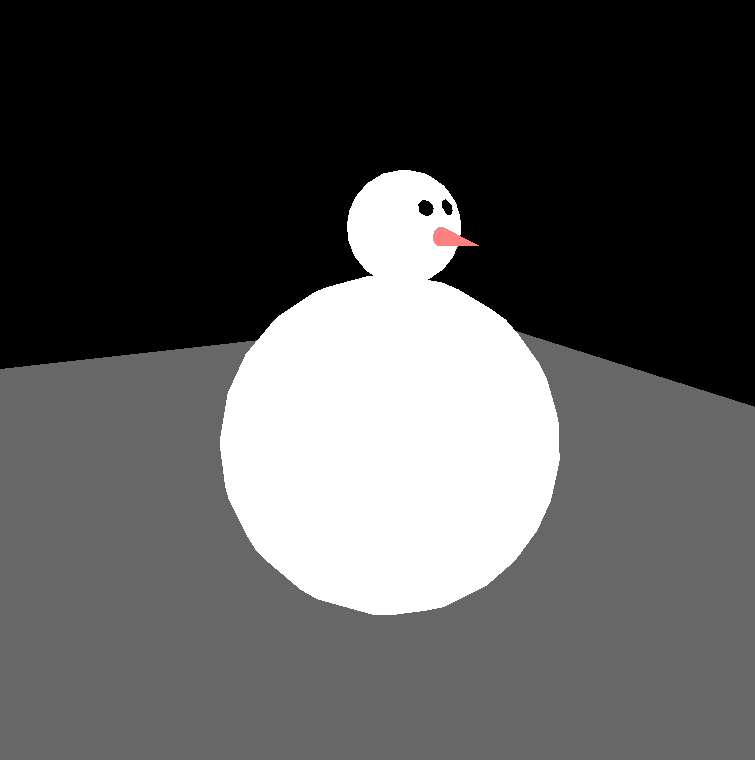
\includegraphics[width=0.9\linewidth]{bonecob.png}
	\caption{Modelagem inicial do boneco de neve}
\end{figure}
	


\subsection{Luz e sombra}

Partindo da imagem modelada do boneco de neve, devemos nesse subtópico vamos detalhar 
a aplicação de sombra e luz, efeitos usados a partir dos mérodos mostrados na
Listing 2.

\begin{lstlisting}[language=Python, caption=Criação e posicionamento da luz]
   
	# Criacao do sombreamento (suave)
    glShadeModel(GL_SMOOTH)

	# Habilita o foco de luz
    glEnable(GL_LIGHTING)

    # Posicionamento do foco da Luz
    lightZeroPosition = [1.0, 4.0, 15.0, 0.]

    # Cor da luz
	lightZeroColor = [0.8, 1.0, 0.8, 1.0]
	
\end{lstlisting}

De acordo com o código descrito, temos a aplicação de uma sombra suave na imagem, depois disso
criamos uma fonte de luz, definimos a sua cor e a posicionamos no cenário de forma a favorecer a forma
do modelo escolhido. Todo esse processo resulta na imagem ilustrada na Figura 2.

\begin{figure}[h]
	\centering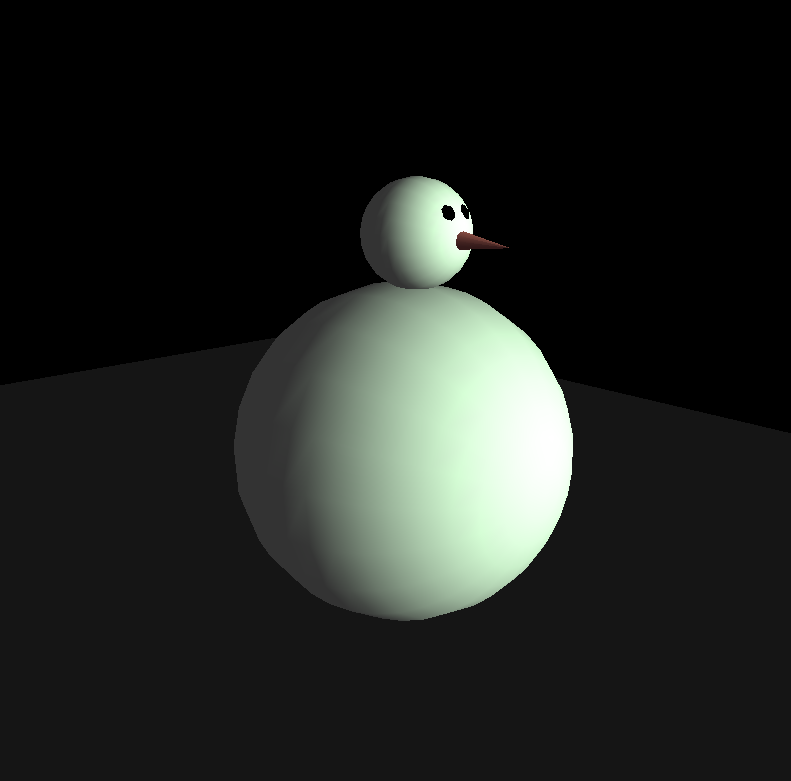
\includegraphics[width=0.9\linewidth]{bonecos.png}
	\caption{Modelagem sombreada do boneco de neve}
\end{figure}

\subsection{Interação}

Buscando gerar uma interação com o usuário a função mostrada no código do Listing 3
é implementada. Esta função tem por finalidade configurar as setas do teclado para que cada uma
delas seja responsável por uma ação.

\begin{lstlisting}[language=Python, caption=Interação com o usuário]
   
	# Metodo que permite utilizar as setas do teclado para rotacionar o boneco
	def controleSetas(key, x, y):
	
		# Para o controle de rotacao vertical
		if(key == GLUT_KEY_UP):
			glRotatef(-1.0, 1.0, 0.0, 0.0)
		elif(key == GLUT_KEY_DOWN):
			glRotatef(1.0, 1.0, 0.0, 0.0)
		# Para o controle de rotacao horizontal
		elif(key == GLUT_KEY_LEFT):
			glRotatef(-1.0, 0.0, 1.0, 0.0)
		elif(key == GLUT_KEY_RIGHT):
			glRotatef(1.0, 0.0, 1.0, 0.0)
	
		glutPostRedisplay()
	
\end{lstlisting}

Definimos então os botões de setas no teclado para que cada um deles execute uma função
correspondente ao movimento direcionado pelo seu descritor. Estes movimentos se dão por funções de rotação.



\section{Conclusão}

Tendo em vista os aspectos descritos e observados nos tópicos e subtópicos desse 
trabalho podemos concluir que a construção de uma representação em 3D exige do programador
um grande conhecimento em técnicas visuais, uma vez que esta representação tem em si um aglomerado
de conceitos que devem ser usados visando uma representação mais próxima possível do real.

Quanto ao algoritmo descrito ao longo deste relatório, podemos destacar o uso do efeito de luz e sombra como
elemento que mais aproximou a representação do boneco de neve em 3D de uma imagem real, uma vez
que a partir dessa aplicação foi notória a mudança visual dada ao objeto.

Além disso, a implementação da interação com o usuário tornou a aplicação mais dinâmica, o que
nos provocou uma maior curiosidade quanto a construção do ambiente. Dado que, a partir dessa interação,
ao executarmos o \textit{script} conseguimos ter a visualização do objeto em todos os pontos.

Por fim, vale destacar a fixação dos conceitos vistos em sala a partir da construção desse projeto,
uma vez que ele nos trouxe a aplicação prática destes conceitos. Ao fim, podemos compreender que ao aplicar um único
conceito ao objeto pode-se causar uma grande modificação na representação visual do mesmo.

\end{document}